% Chapter Template

\chapter{Results} % Main chapter title
\label{chap:results}


%B-Feld. Von welchem Instrument? auch RTN-System. Genauso Winkel berechnet.
%1-min-Mittel (Gyroradius Zeit zeigen) und entsprechend EpQ-Steps den PHAs zugeordnet.

%
%
%
Todo:\\
Schreiben, dass die velocity Akzeptanzpunkte mit den anteilmäßigen Counts histogrammiert werden? Vielleicht auch ins Data-Kapitel, weil das mit der Normierung gemacht wird...? Sind die Counts überhaupt durch n geteilt?\\ \\
\textbf{Steps vsw, asp...?}
\\ \\ \\
Here we present the results of the procedure described in chapter \ref{chapter:data}. For creating HE+ VDs from He+ SWICS PHA data we synchronize the selected data (s. \ref{chapter:instrumentation} (triple coincidences) with the SC AA, eigen-velocity and solar wind speed.
This gives us directionally resolved counts from the observed phase space volume.
\\
An example for todo days bla is shown in fig. \ref{fig:counts_50}. Here we histogrammed the counts by utilizing cartesian $w_R$, $w_T$ and $w_N$ bins in solar wind frame. Shown are counts in the $w_T - w_N$ plane from a ``slice'' that has been cut out in $w_R$ direction. The orientation of such a cut is sketched in fig. \ref{fig:sketch_slice_R}. In fig. \ref{fig:counts_50} counts within the range $0.3 <= w_R < 0.5$ have been summarized for each $w_T - w_N$ bin.
(D.h. bei vsw ...)
\\
Dividing the counts by the integrated phase space volume for the observed time, which is binned in the same way and shown in fig. \ref{fig:norm_50}, gives the resulting phase space density, s. fig. \ref{fig:psd_50}.\\
When comparing the three figures one can see a change in shape between phase space volume and phase space density (resp. counts). The phase space density does not cover all of the scanned phase space volume. This means that SWICS did not observe He+ pickup ions over all of the observed phase space volume but only in a distinct partial volume.\\ 
The non-zero parts of phase space density show as a roundish shape in the 2D projection in fig todo. In fact, it is a spherical shape in 3D. As a visualization a stepwise sequence of $w_T - w_N$ ``slices'' is shown in the appendix. Each slice is again a projection of the psd from a width $\Delta w = 0.2$. The sequence starts at about solar wind speed with the slice $-0.1 <= w_R < 0.1 todo$ and steps seamlessly up to $0.9 <= w_R < 1.1$ in todo increments. The radius of the projection decreases towards larger $w_R$ which suggests the 3d shape of a sphere centered around $w_R = 0$.
For $w_R < 0$ and towards smaller values of $w_R$ an increasing ``hole'' in the phase space density emerges from the center. This is due to the fact of a limited instrumental coverage for He at higher ESA steps, which is described in more detail in todo.\\ The same shape shows up when taking slices in the other two dimensions. Verweis auf beide Spektren und die Skizzen.\\

Looking again at the $0.9 <= w_R < 1.1$ slice in fig todo one observes.
Also, the psv shosw a deutlich, schmalen peak in the bins around wT = todo and wN = todo. This means that this part of ps has been observed more often than surrounding parts. This is due to the fact that the spacecraft had a substantial (?) aspect angle (vgl bild bla) in this period of time. Which means that the sc's spin axis for most of the time was tilted away from the radial direction which is reflected by the fact that the peak is shifted a little bit away form the center.The fact that this distinct psv has been observed especially often is followed by a qualitatively similar peak in counts (s. fig todo). 
This is a result of the measurement and not a feature in the velocity distribution of he+. In PSD that feature has vanished, which shows the importance of normalization process. The PSD shows an increased density over a wider range around the radial direction, majority streams central in this example. \\ \\
In fig todo we show the psd for another longer time period todo for slice todo at vsw todo. Here, the counts show a ring structure which vanishes by normalization. 
The PSD in fig todo shows a similar distribution like the psd from the other time period, concentrated and symmetrical around central direction.
\\ \\
Of course we are not limited to the presented Cartesian projections.
We can also choose a shell-wise projections. For this we consider spherical shells of constant $w$ in sw frame. Visualization: fig todo: 2d projection of such a concentric shell around w = 0 is shown. Irgendwo Winkel einzeichnen oder erklären.
\\
Graue Fläche kurz erklären
\\
In Figs. \ref{fig:sky_counts} and \ref{fig:sky_norm} we show counts and integrated phase space volume in such a projection for $\mathrm{He^{+}}$ measurements from 50 days 1993, restricted to solar wind speeds from $760 \, \mathrm{km\,s^{-1}}$ to $780 \, \mathrm{km\,s^{-1}}$. The selected spherical shell comprises absolute $w$-values $0.85 <= w < 0.95$. Even more clearly than in bla clearly peaks at bla are apparent in both figures, which is due to the variation in observation time of distinct phase space volumes. The histogram of the corresponding phase space density, that excludes this effect, is shown in figure bla.
This projection can become particularly suitable for the examination of the level of isotropy within a $w$-shell. Shapes like a torus distribution (ref PUI Kapitel) could be observed directly. For a completely isotropized shell we would expect an evenly colored projection in Fig todo. This is obviously not the case. Here, we find a structure of increased phase space density that is around $-60\,^\circ$ longitude for $\vartheta = 0\,^\circ$ and moves towards $\varphi = 0\,^\circ$ for higher latitudes.
\\
Unfortunately, we could not find clear structures that were constant over different periods of measurement. A possible reason for that could be that the detection efficiency in chap todo could only have been determined very vaguely. As the shell projection comprises measurements from different ESA steps (s. Zeichnung todo), an inaccurate efficiency weighting could either lead to a disappearance of real structures or even to an emerging of artificial ones. A detailed analysis of the detection efficiencies like it is shown in \citet{koeten} for ACE/SWICS is beyond the scope of this work but would be highly beneficial for future analyses.


.
\\ \\
In Fig todo we show 1D projections of 3D VDF from measurements of two different years. In each year (1994, 1996) we analyzed $\mathrm{He^{+}}$ data from 100 days at solar wind speeds from $760 \, \mathrm{km\,s^{-1}}$ to $770 \, \mathrm{km\,s^{-1}}$. 

For this projection we integrate both the counts and the phase space volume over spherical shells around $w=0$. In a 2D projection this can be visualized by a integration along a blue circle in Fig. todo. We combined values within the width $\Delta w = 0.1$ at different radii from $w = 0.25$ to $w = 1.05$. In Fig todo the histogram of the resulting PSD is shown.
The histograms look qualitatively similar for both years. 
We see a relatively broad distribution with a clear cutoff around $w = 1$ which corresponds to $w_{SC} = 2$ (Verweis PUI Kapitel). For smaller values of $w$ the distribution does not change over many magnitudes. 


The spectra in Fig. todo are also in good qualitative agreement with the one in Fig.(todo:gloeckler). It should be noted that our spectra are limited to values $w > 0.25$, while the spectrum in todo is continued down to values $w_{SC} < 1$, which corresponds to values $w < 0$ in solar wind frame. 
In sec todo we have seen that He+ Triple Coincidences can only be measured for distinct $w$-values above a limit that is dependant on the solar wind speed but hardly smaller than $w = 1$. This shows that the spectrum in Fig.(todo:gloeckler) is not based on solely Triple Coincidences but also on He+ Double Coincidences. As Double Coincidences lack an energy measurement in the solid-state detector and thus a directional resolution, the spectrum can only result from an integration along different ESA shells that is projected onto a distinct possible value.
\\
Although the spectra look similar we want to emphasize that the spectrum in Fig. todo results from a very different approach as we show projected cuts through an actual three dimensional velocity distribution.

\clearpage
\subsection{Slices}


%%% R %%%

\begin{figure}[h]
	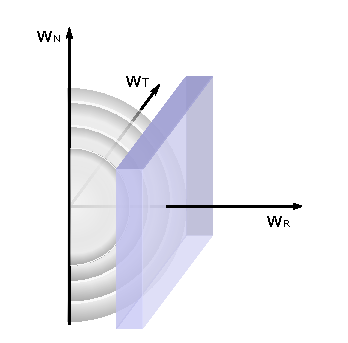
\includegraphics[width=.4\textwidth]{Figures/sketch_slice_R2.pdf}
	\centering
	\caption{todo}
	\label{fig:sketch_slice_R}
\end{figure}


\begin{figure}
	\centering
	\begin{subfigure}{.5\textwidth}
		\centering
		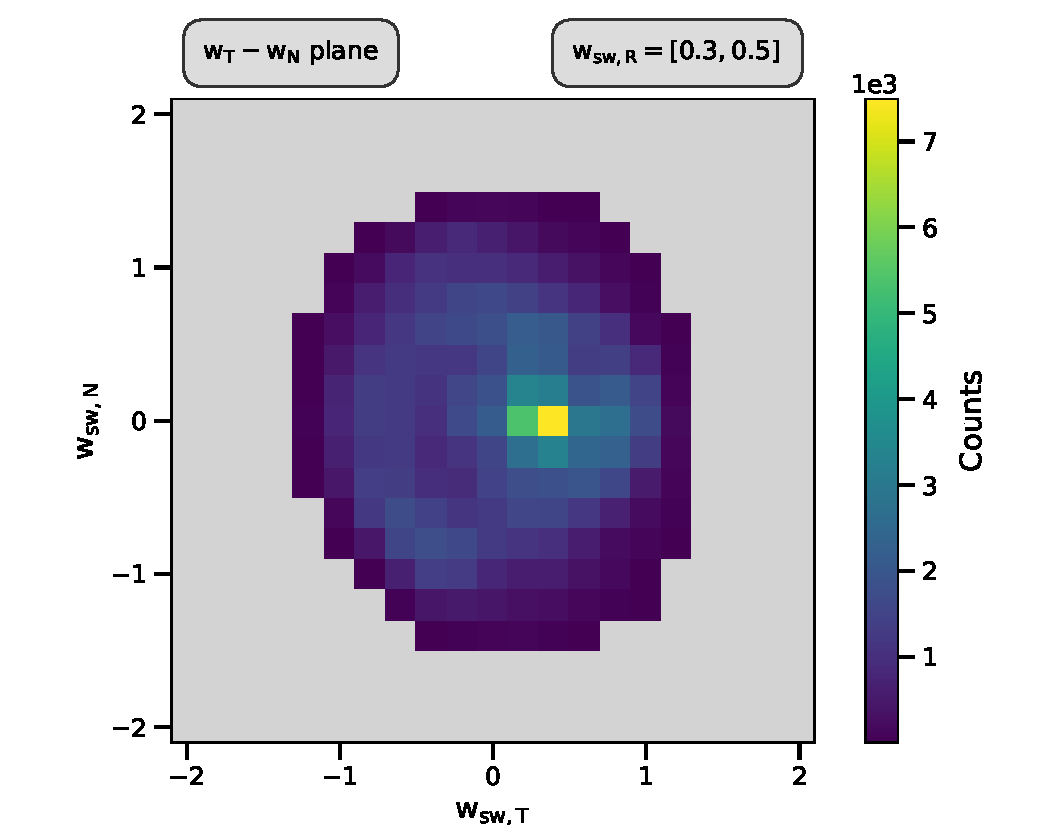
\includegraphics[width=1\textwidth]{Figures/slice_50_counts.pdf}
	\end{subfigure}%
	\begin{subfigure}{.5\textwidth}
		\centering
		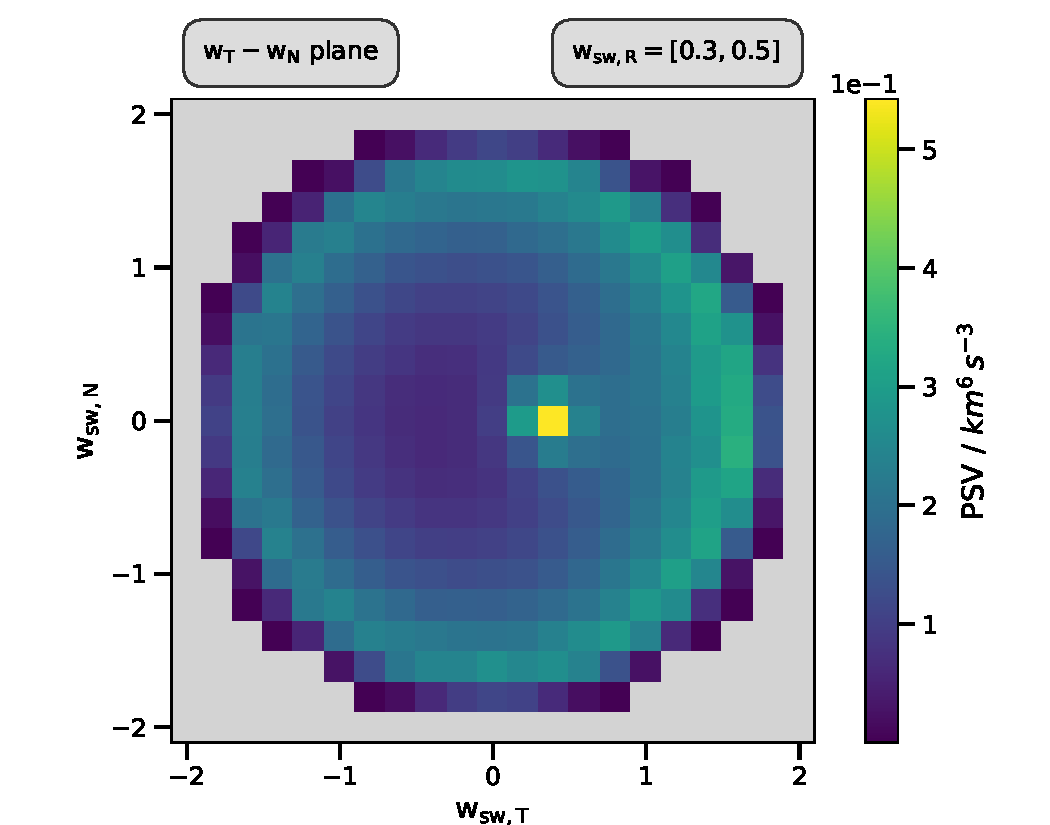
\includegraphics[width=1\textwidth]{Figures/slice_50_norm.pdf}
	\end{subfigure}
	\caption{ring in norm due to psv auf anderen Schalen; da größere Volumina wegen v}
	\label{fig:counts_norm_50}
\end{figure}



\begin{figure}[h]
	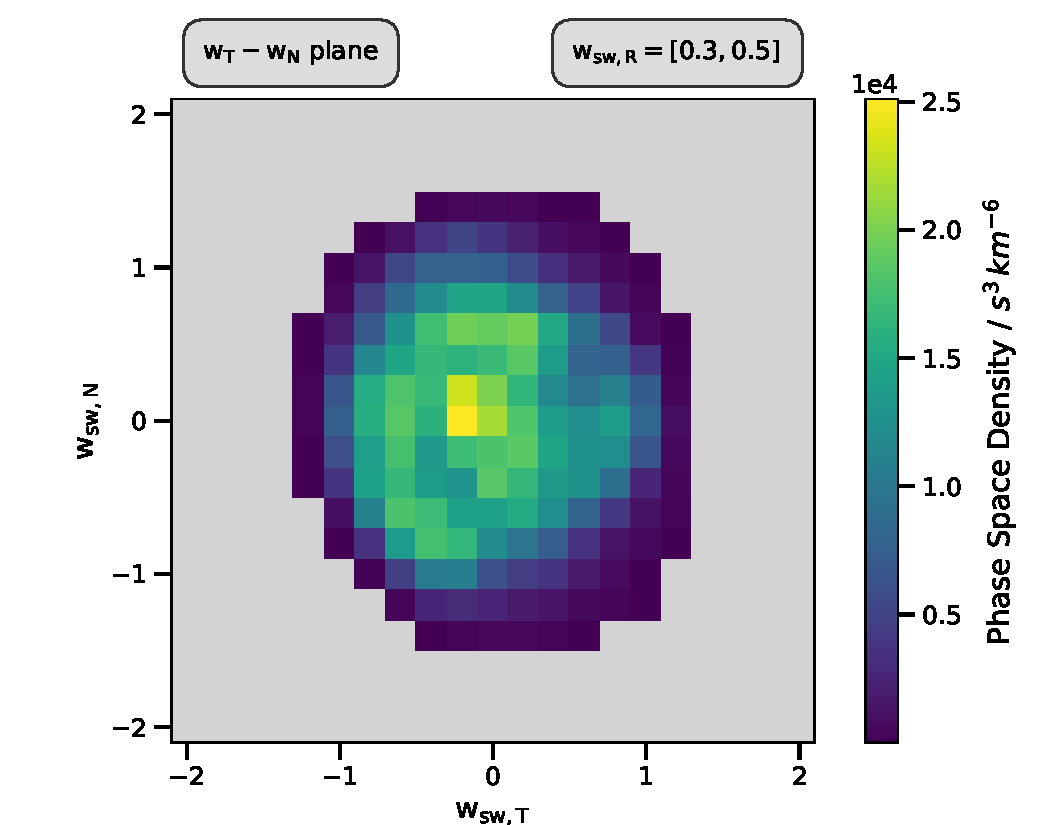
\includegraphics[width=.8\textwidth]{Figures/slices_50_3.pdf}
	\centering
	\caption{todo}
	\label{fig:psd_50}
\end{figure}


\begin{figure}
	\centering
	\begin{subfigure}{.5\textwidth}
		\centering
		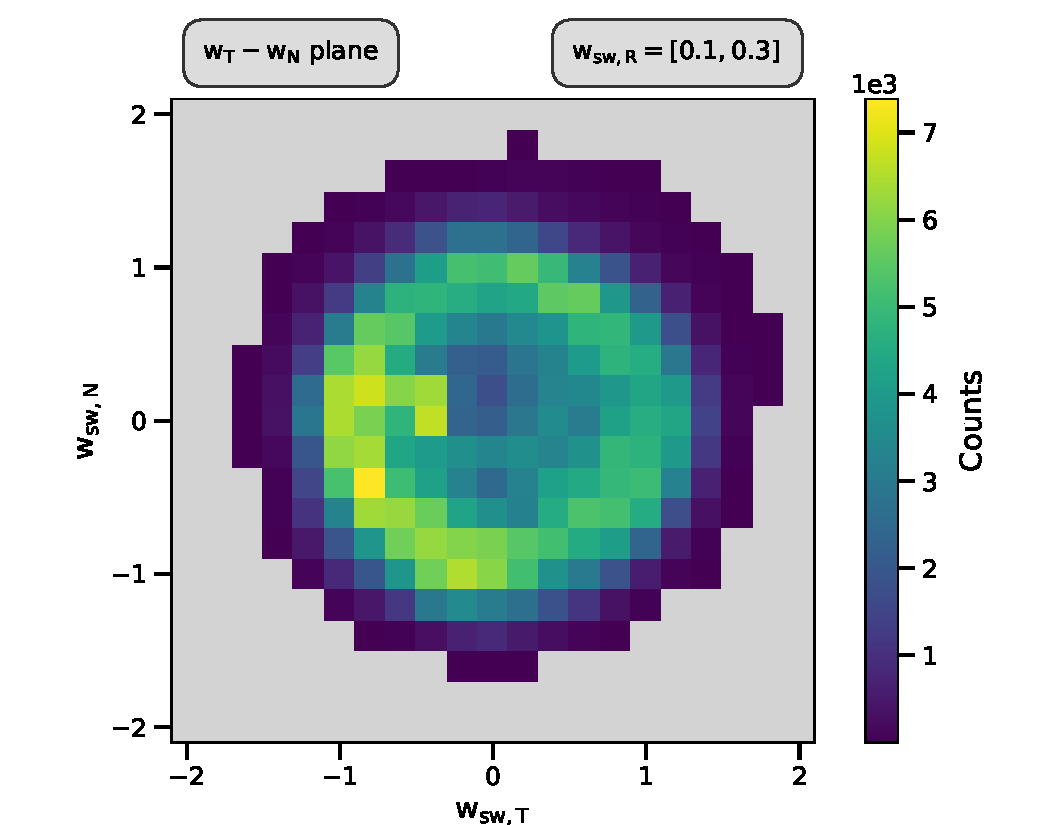
\includegraphics[width=1\textwidth]{Figures/cart_long_counts.pdf}
	\end{subfigure}%
	\begin{subfigure}{.5\textwidth}
		\centering
		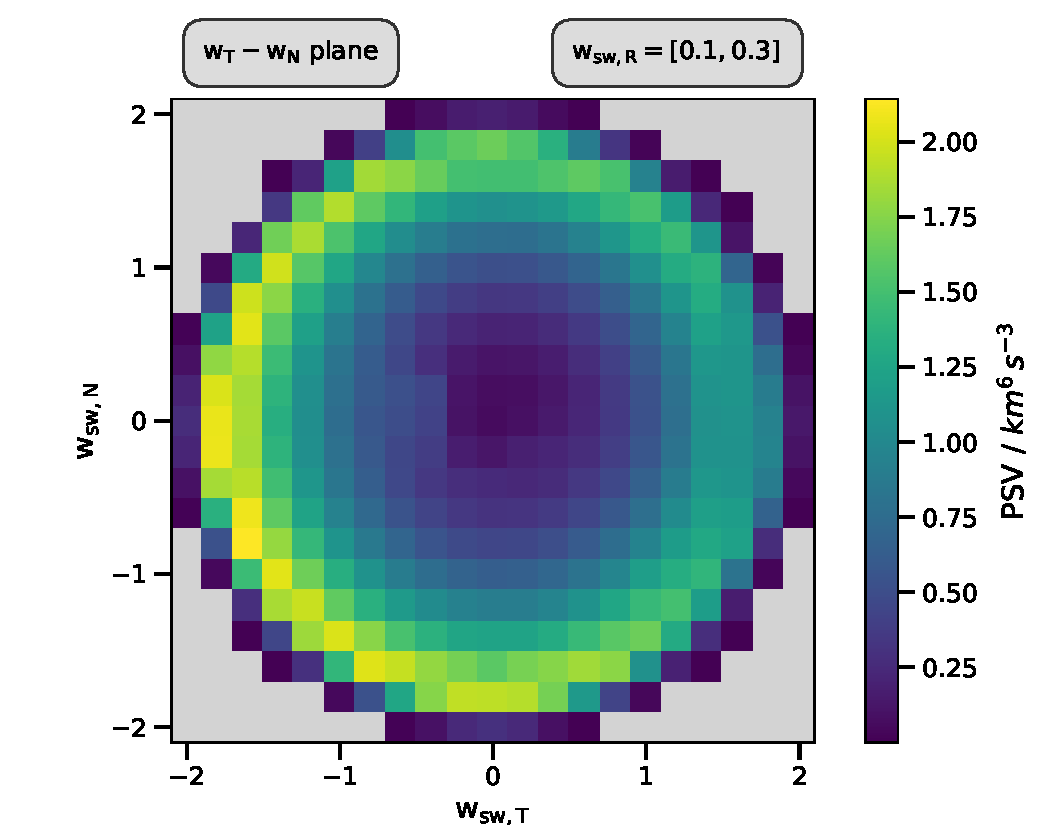
\includegraphics[width=1\textwidth]{Figures/cart_long_norm.pdf}
	\end{subfigure}
	\caption{todo}
	\label{fig:counts_norm_lang}
\end{figure}


\begin{figure}[h]
	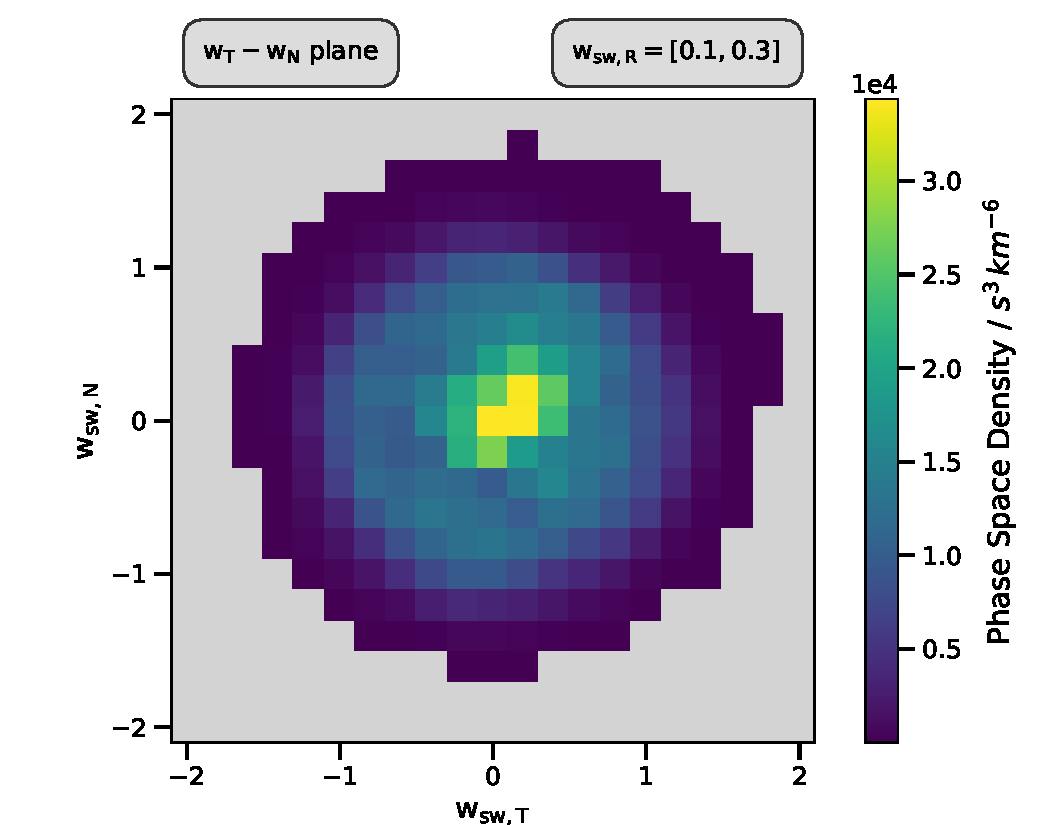
\includegraphics[width=.8\textwidth]{Figures/cart_long_ps.pdf}
	\centering
	\caption{todo}
	\label{fig:psd_lang}
\end{figure}






%%% T %%%
\begin{figure}[h]
	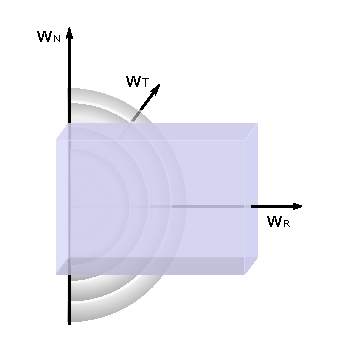
\includegraphics[width=.4\textwidth]{Figures/sketch_slice_T2.pdf}
	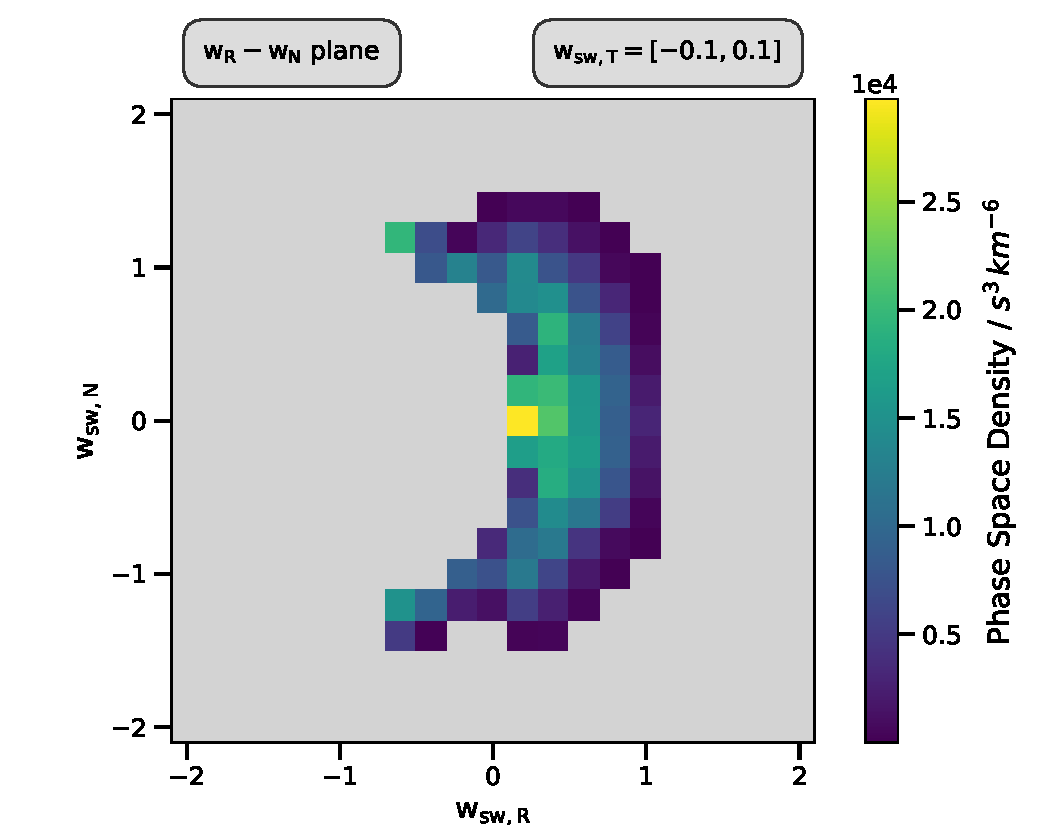
\includegraphics[scale=.45]{Figures/slice_50_T.pdf}
	\centering
	\caption{todo}
	\label{fig:sketch_slice_T}
\end{figure}

%%% N %%%

\begin{figure}[h]
	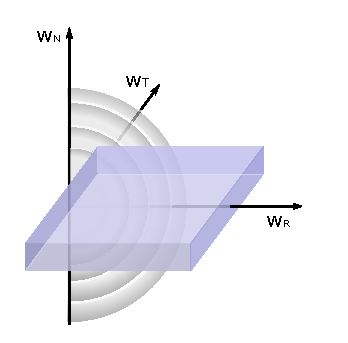
\includegraphics[width=.4\textwidth]{Figures/sketch_slice_N2.pdf}
	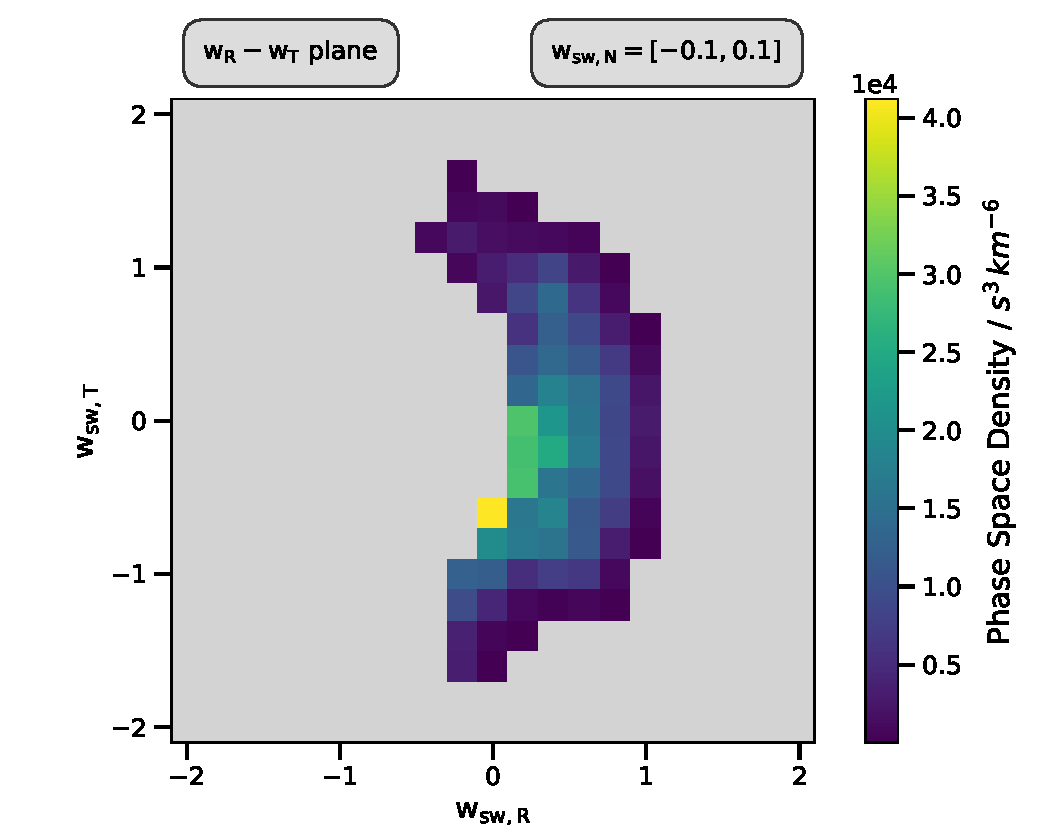
\includegraphics[scale=.45]{Figures/slice_50_N.pdf}
	\centering
	\caption{todo}
	\label{fig:sketch_slice_N}
\end{figure}


%
%
%
\clearpage
\subsection{Skymaps}
\begin{figure}[h]
	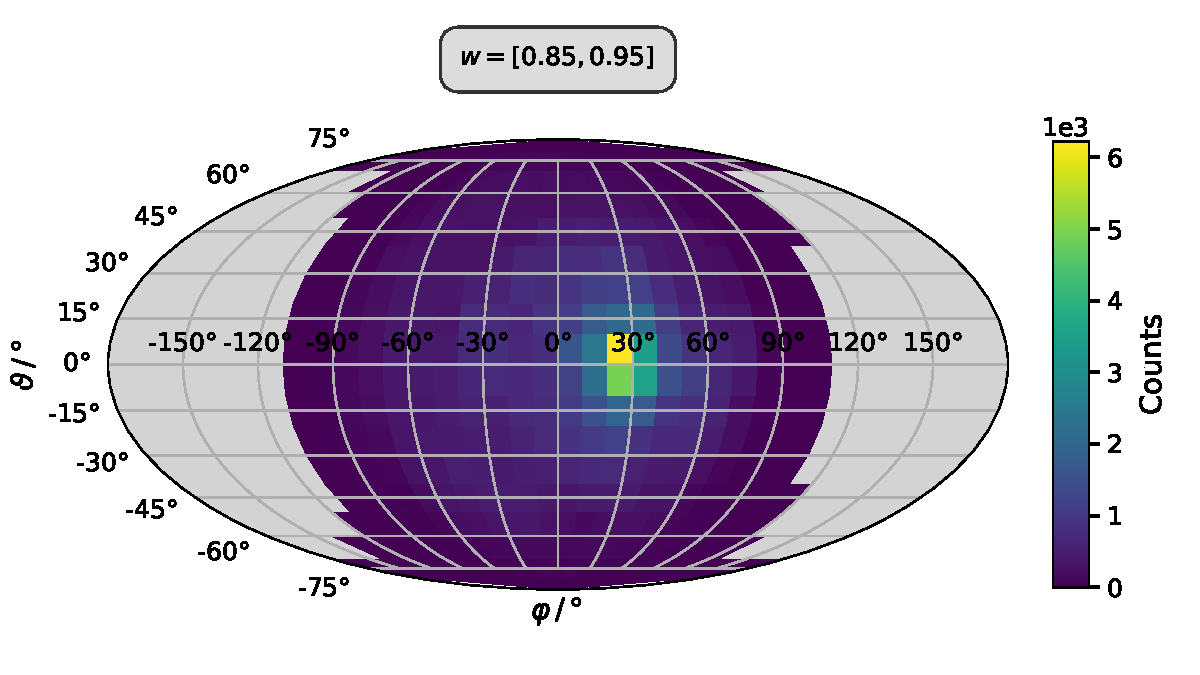
\includegraphics[width=1\textwidth]{Figures/sky_counts.pdf}
	\centering
	\caption{todo}
	\label{fig:sky_counts}
\end{figure}
\begin{figure}[h]
	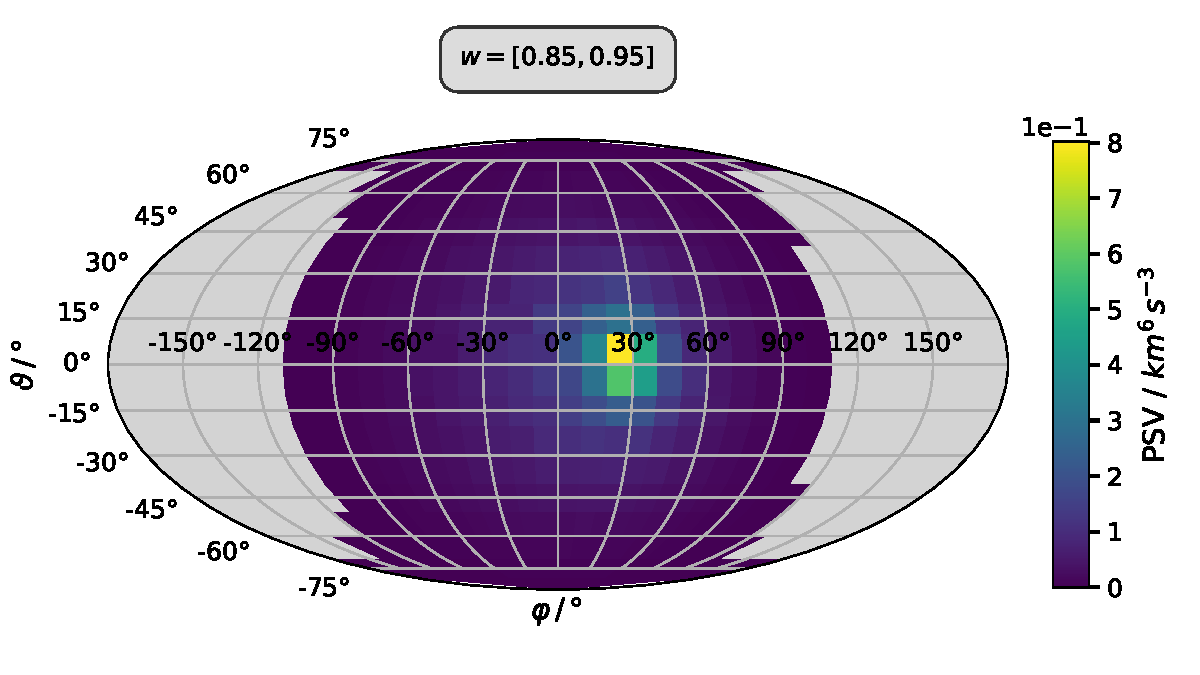
\includegraphics[width=1\textwidth]{Figures/sky_norm.pdf}
	\centering
	\caption{todo}
	\label{fig:sky_norm}
\end{figure}
\begin{figure}[h]
	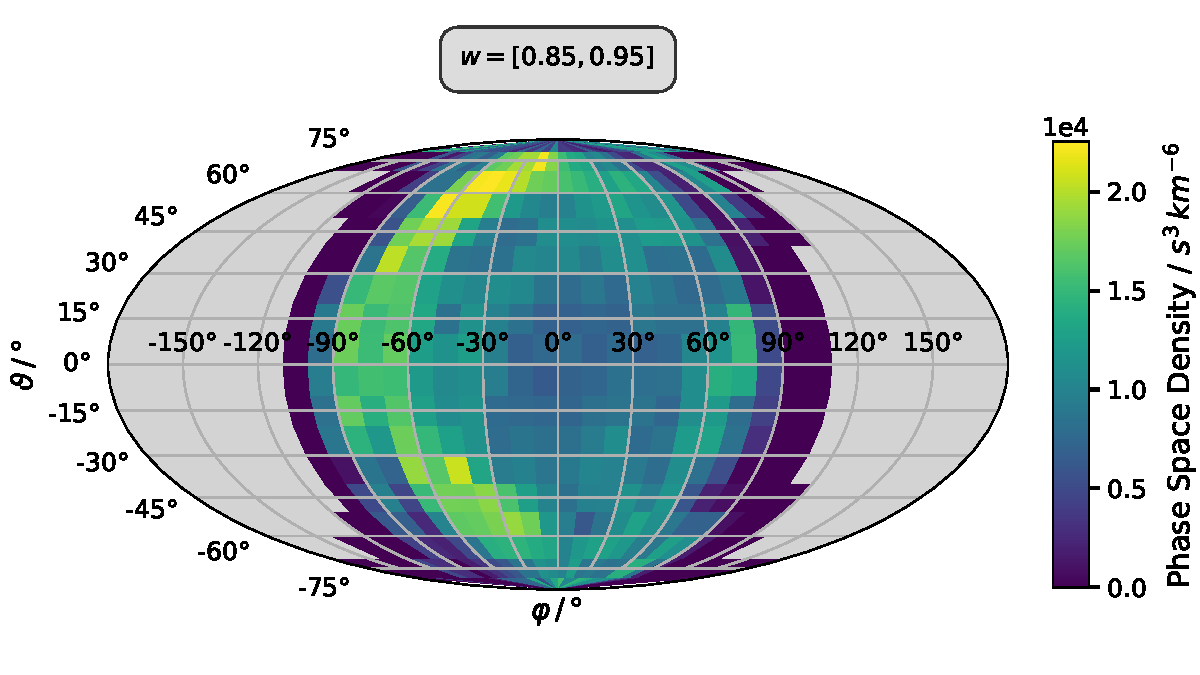
\includegraphics[width=1\textwidth]{Figures/sky_ps.pdf}
	\centering
	\caption{todo}
	\label{fig:sky_psd}
\end{figure}
%
%
%
\clearpage
\subsection{1D}

\begin{figure}[h]
	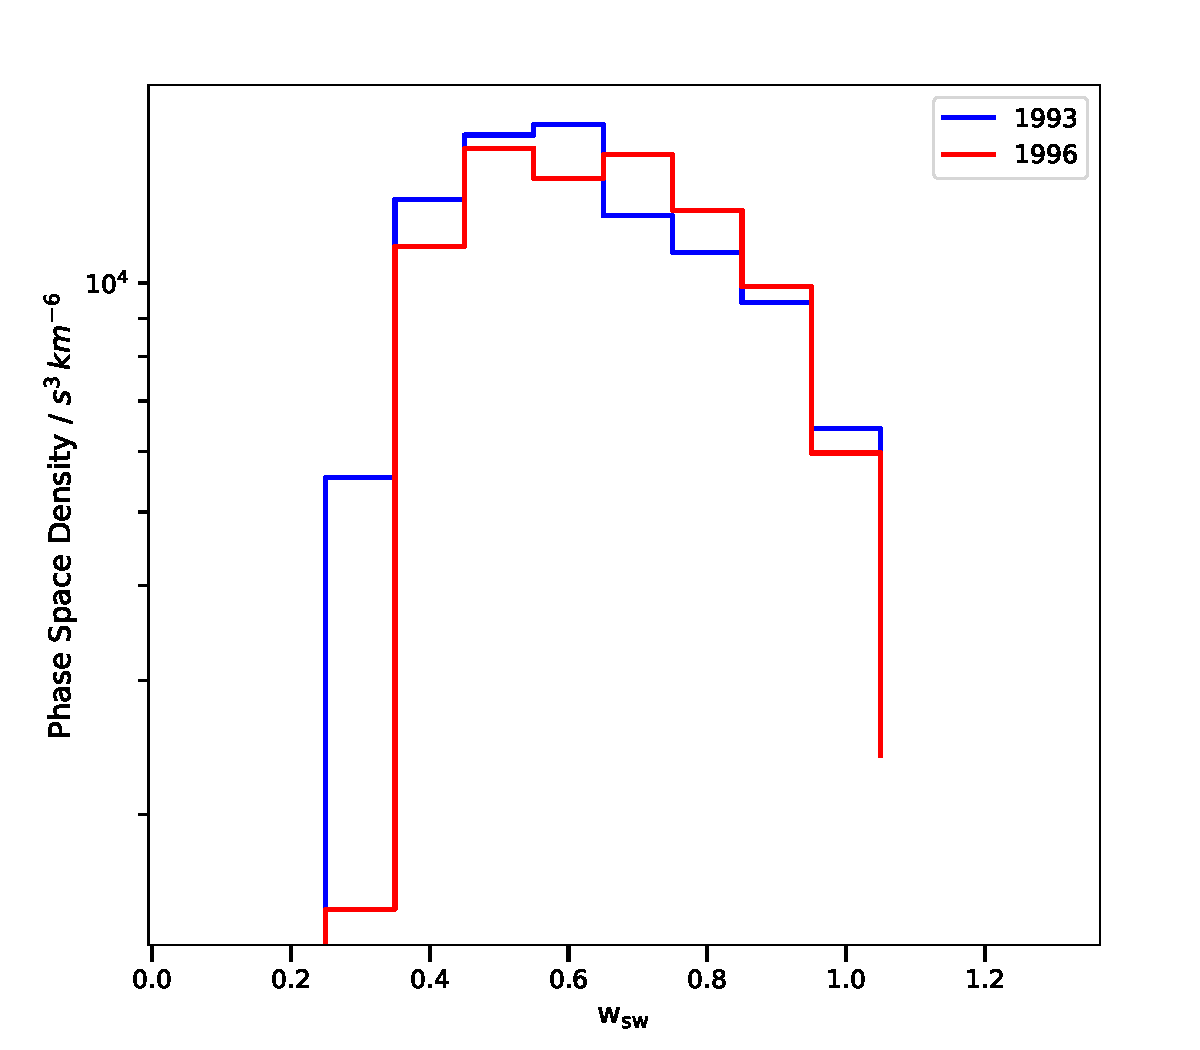
\includegraphics[width=.8\textwidth]{Figures/1D.pdf}
	\centering
	\caption{todo}
	\label{fig:todo}
\end{figure}

%
%
%
\clearpage
\section{Loose Ends}
\begin{itemize}
	\item andere Daten: B, vsw (Swoops: als vsw wird Protonengeschw. genommen. Ist das überhaupt richtig, ist das der Referenzframe? Und Annahme, dass vsw rein radial ist)
	\item Die Sache mit dem BRW ab 2003
	\item Englisch: Relativpronomen, Kommasetzung, British/American
	\item $\mathrm{He^{+}}$ einheitlich, mathrm
	\item Tempus?
	\item kursiv / nicht kursiv wie war das nochmal
	\item spinrate drin?
\end{itemize}
